% !TeX encoding = UTF-8
% !TeX spellcheck = en_US
% !TeX root = ../../Thesis.tex

\chapter{Deflection Electronics}

\begin{figure}
	\centering
	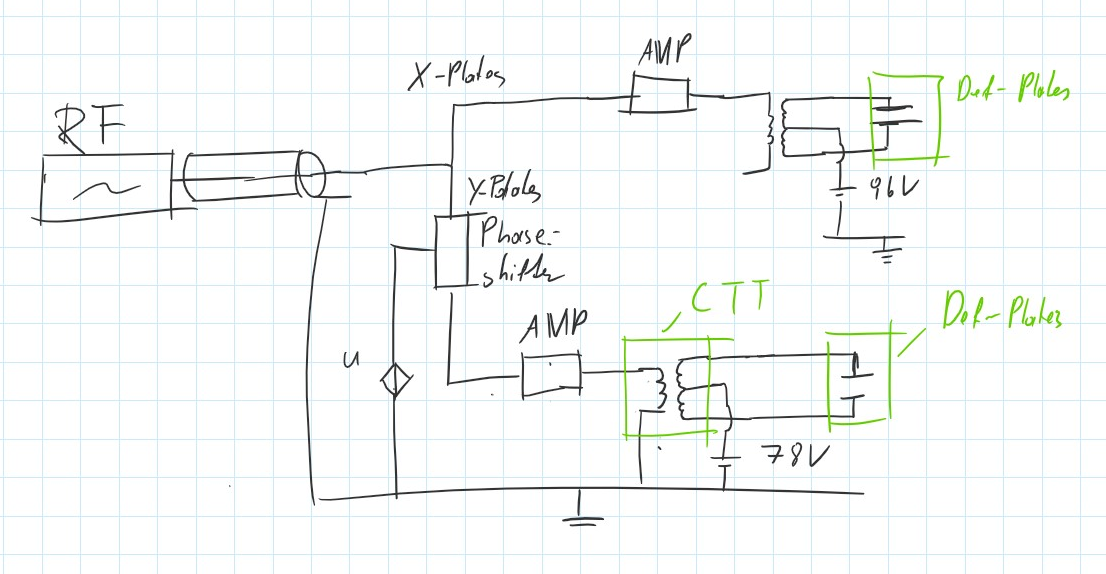
\includegraphics[width=0.7\linewidth]{Chapters/Deflection/deflec_circuit}
	\caption{Deflection circuit}
	\label{fig:defleccircuit}
\end{figure}

\begin{figure}
	\centering
	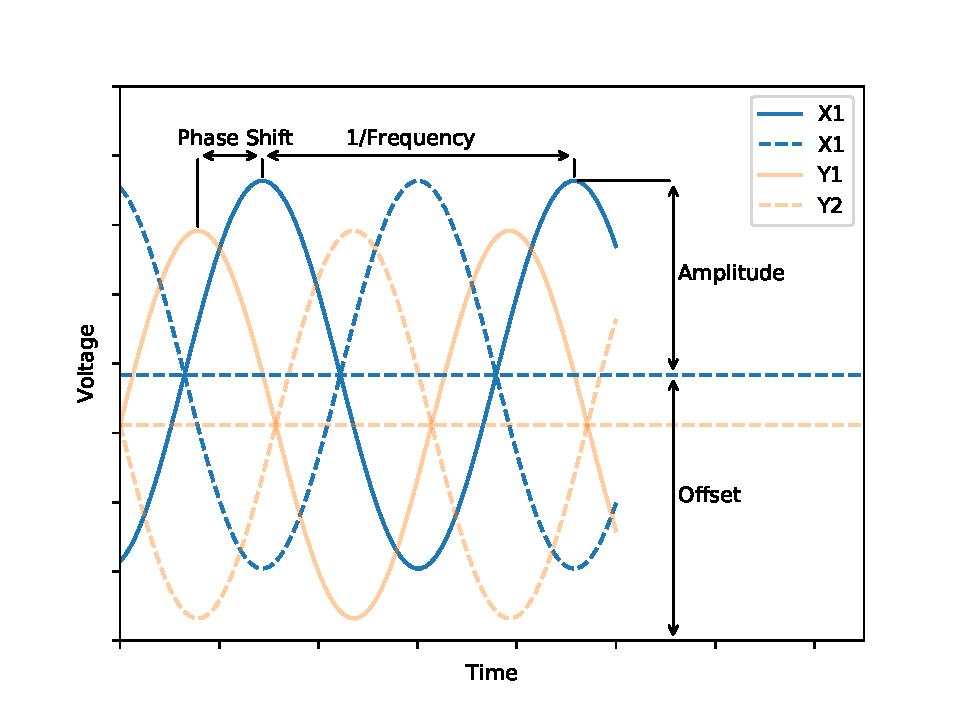
\includegraphics[width=0.7\linewidth]{Chapters/Deflection/VoltageAspects}
	\caption{}
	\label{fig:VoltageAspects}
\end{figure}

\begin{figure}
	\centering
	\includegraphics[width=0.7\linewidth]{Chapters/Deflection/Lissajous}
	\caption{ from \cite{Wikipedia Lissajous}}
	\label{fig:Lissajous}
\end{figure}






\begin{figure}
	\centering
	\begin{subfigure}{.5\textwidth}
		\centering
		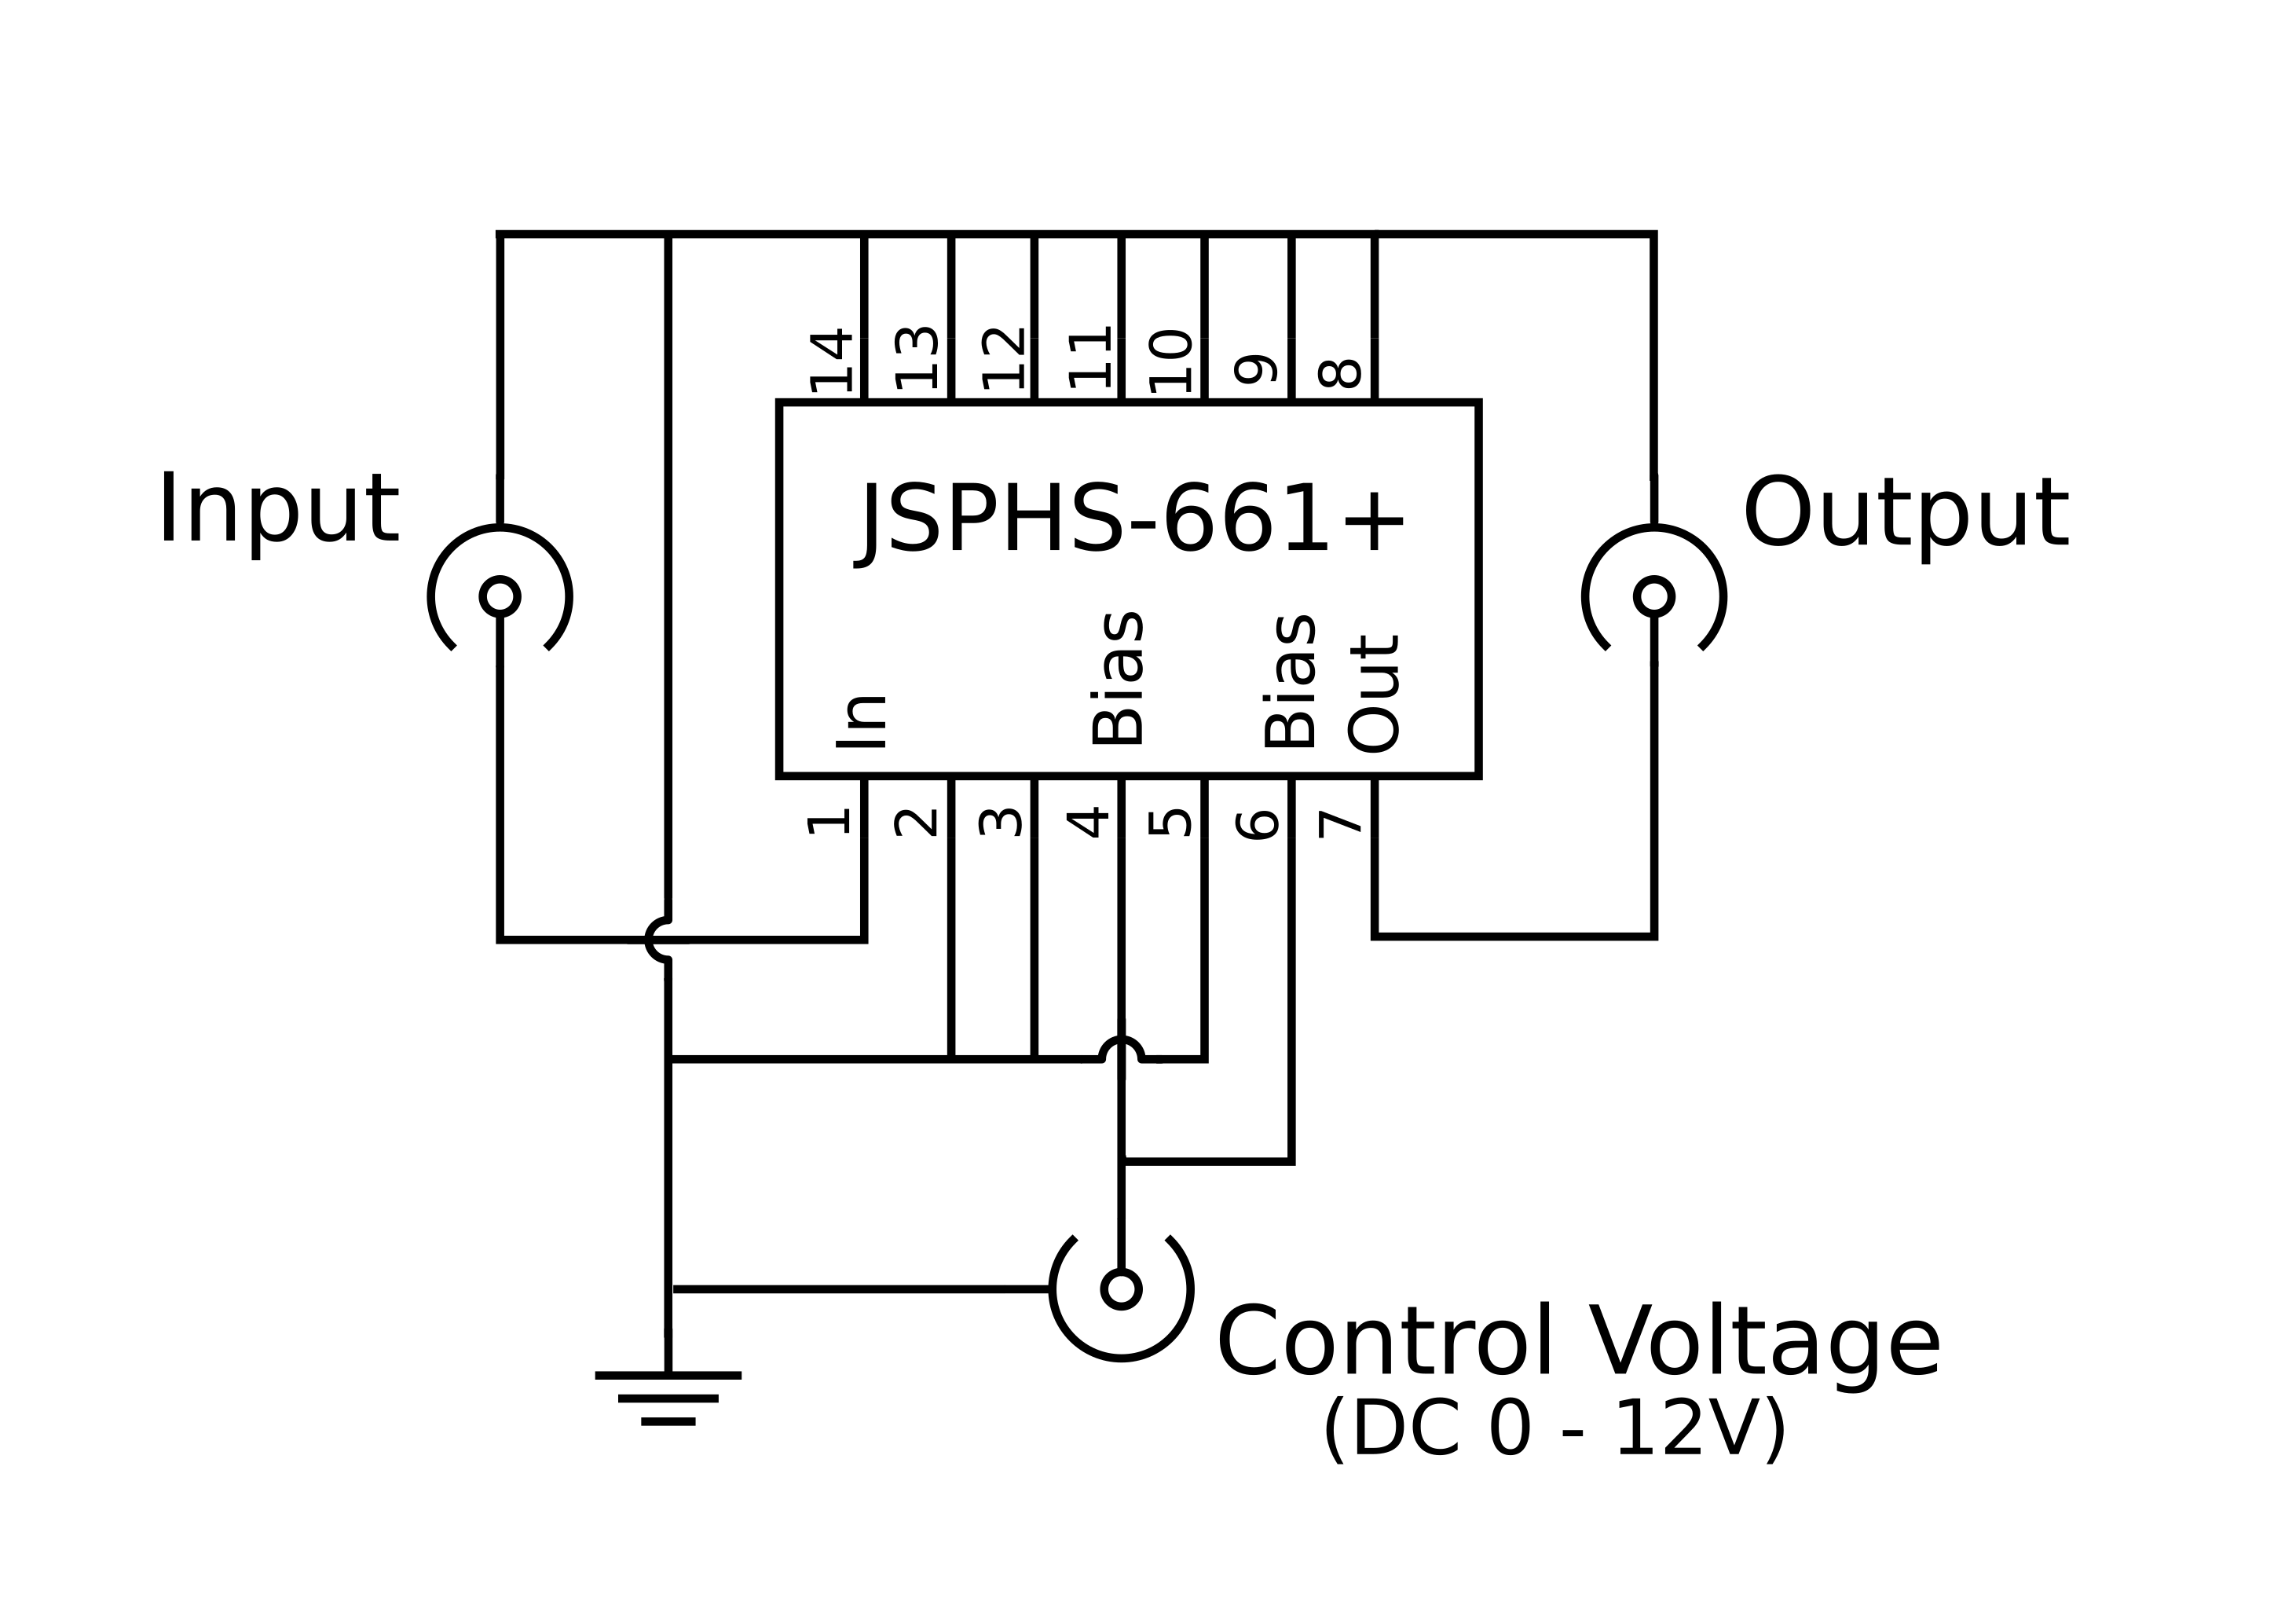
\includegraphics[height=0.2\textheight]{Chapters/Deflection/circuit_phase}
		\caption{}
		\label{fig:circuit_phase}
	\end{subfigure}%
	\begin{subfigure}{.5\textwidth}
		\centering
		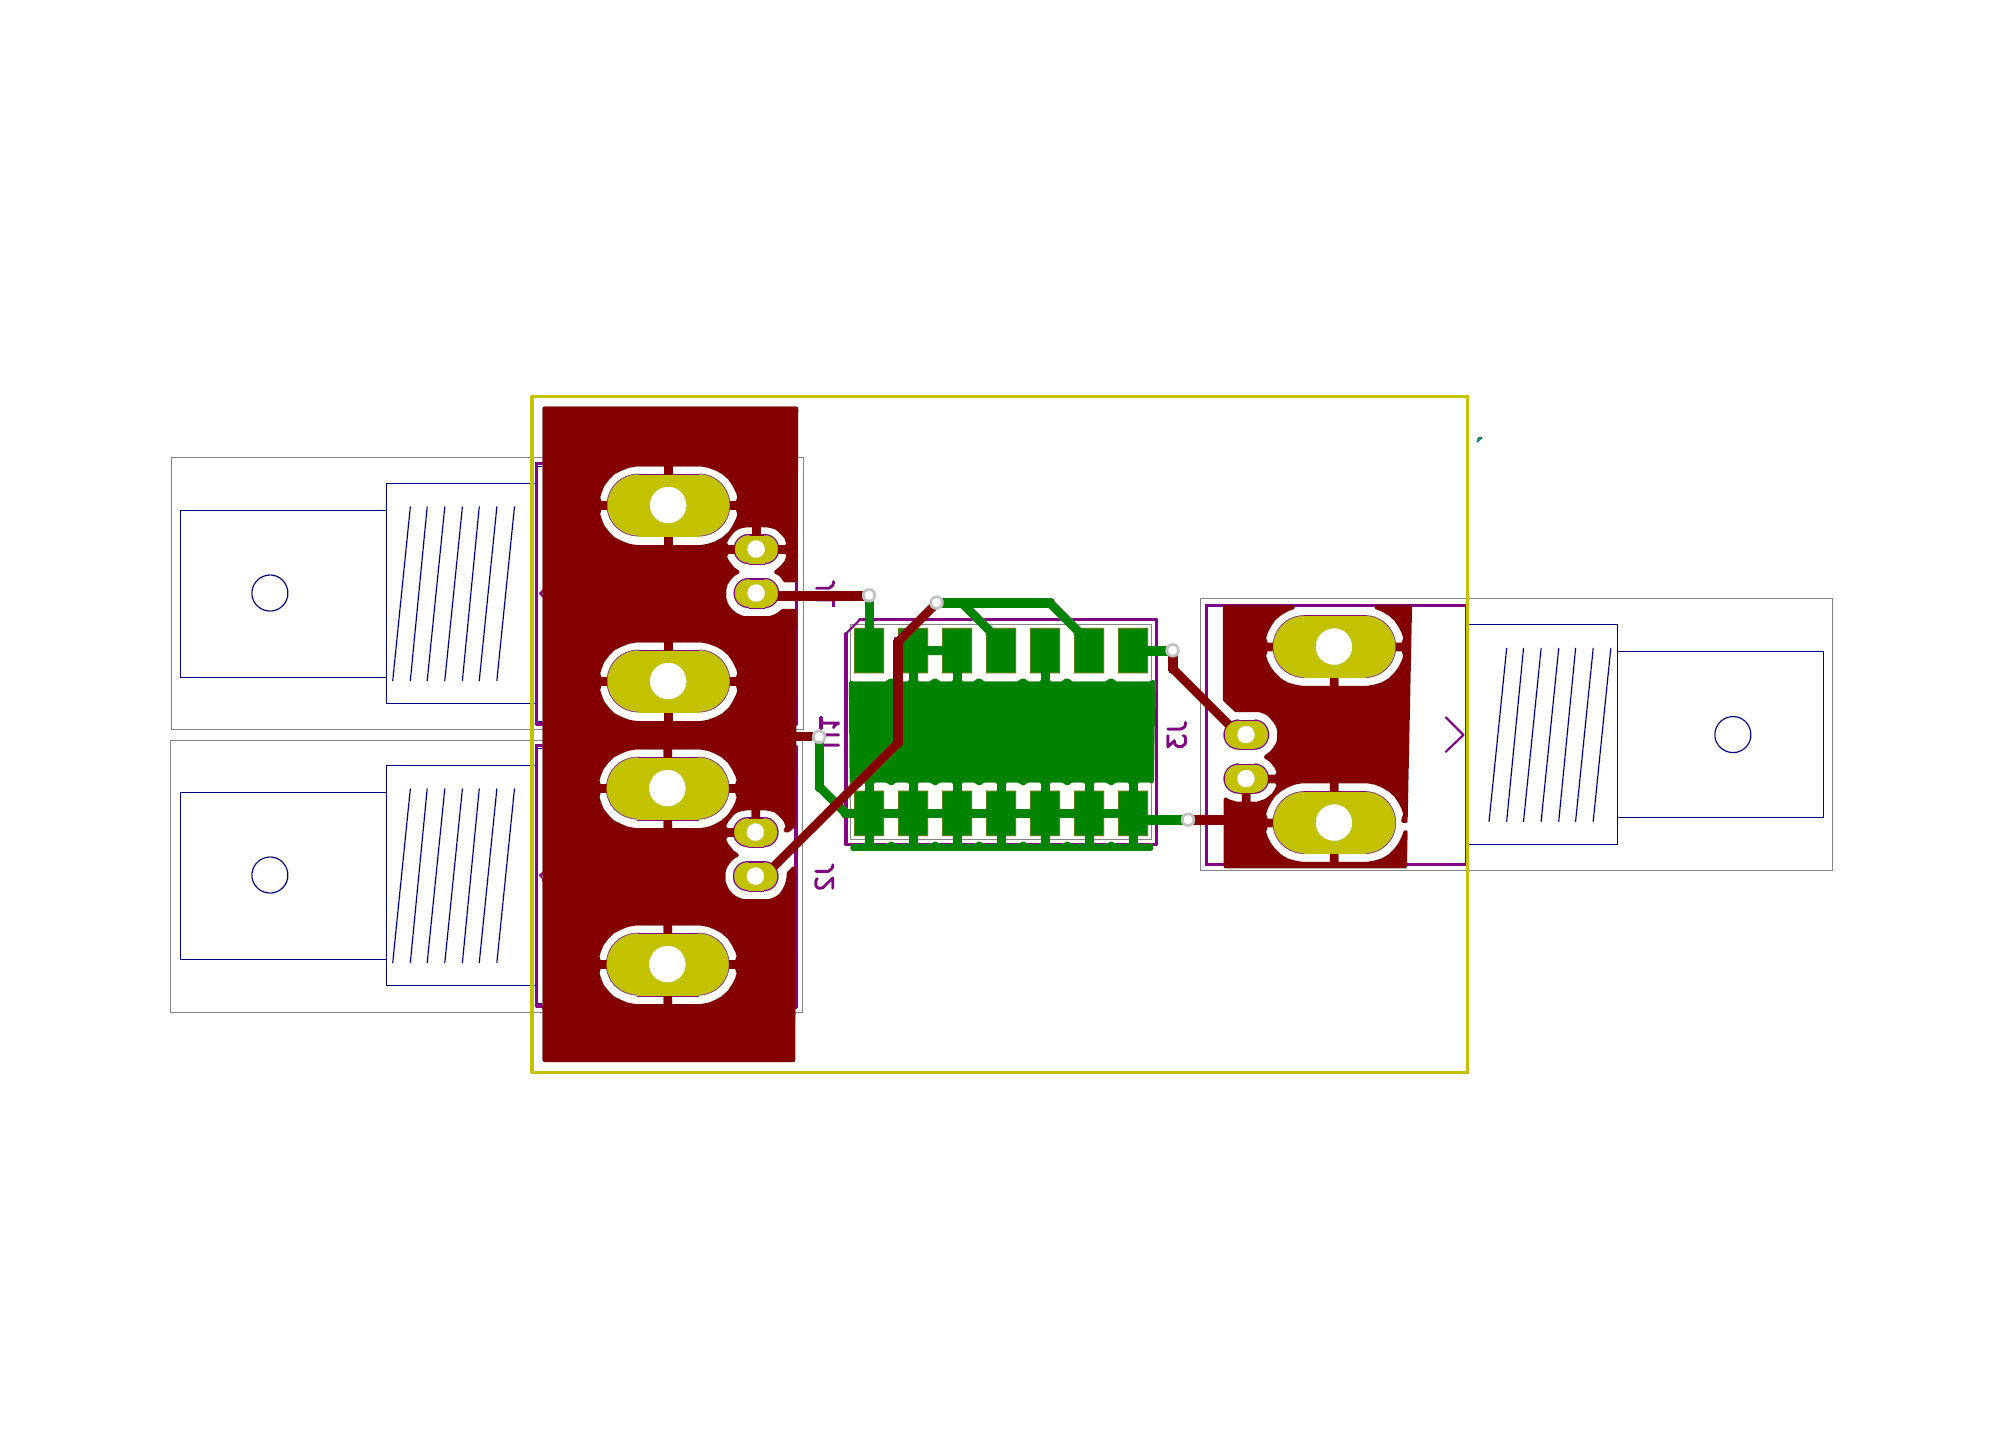
\includegraphics[height=0.2\textheight]{Chapters/Deflection/PCB_phase}
		\caption{}
		\label{fig:PCB_phase}
	\end{subfigure}
	\caption{}
	\label{fig:PhaseShifter}
\end{figure}

\begin{figure}
\centering
\begin{subfigure}{.5\textwidth}
	\centering
	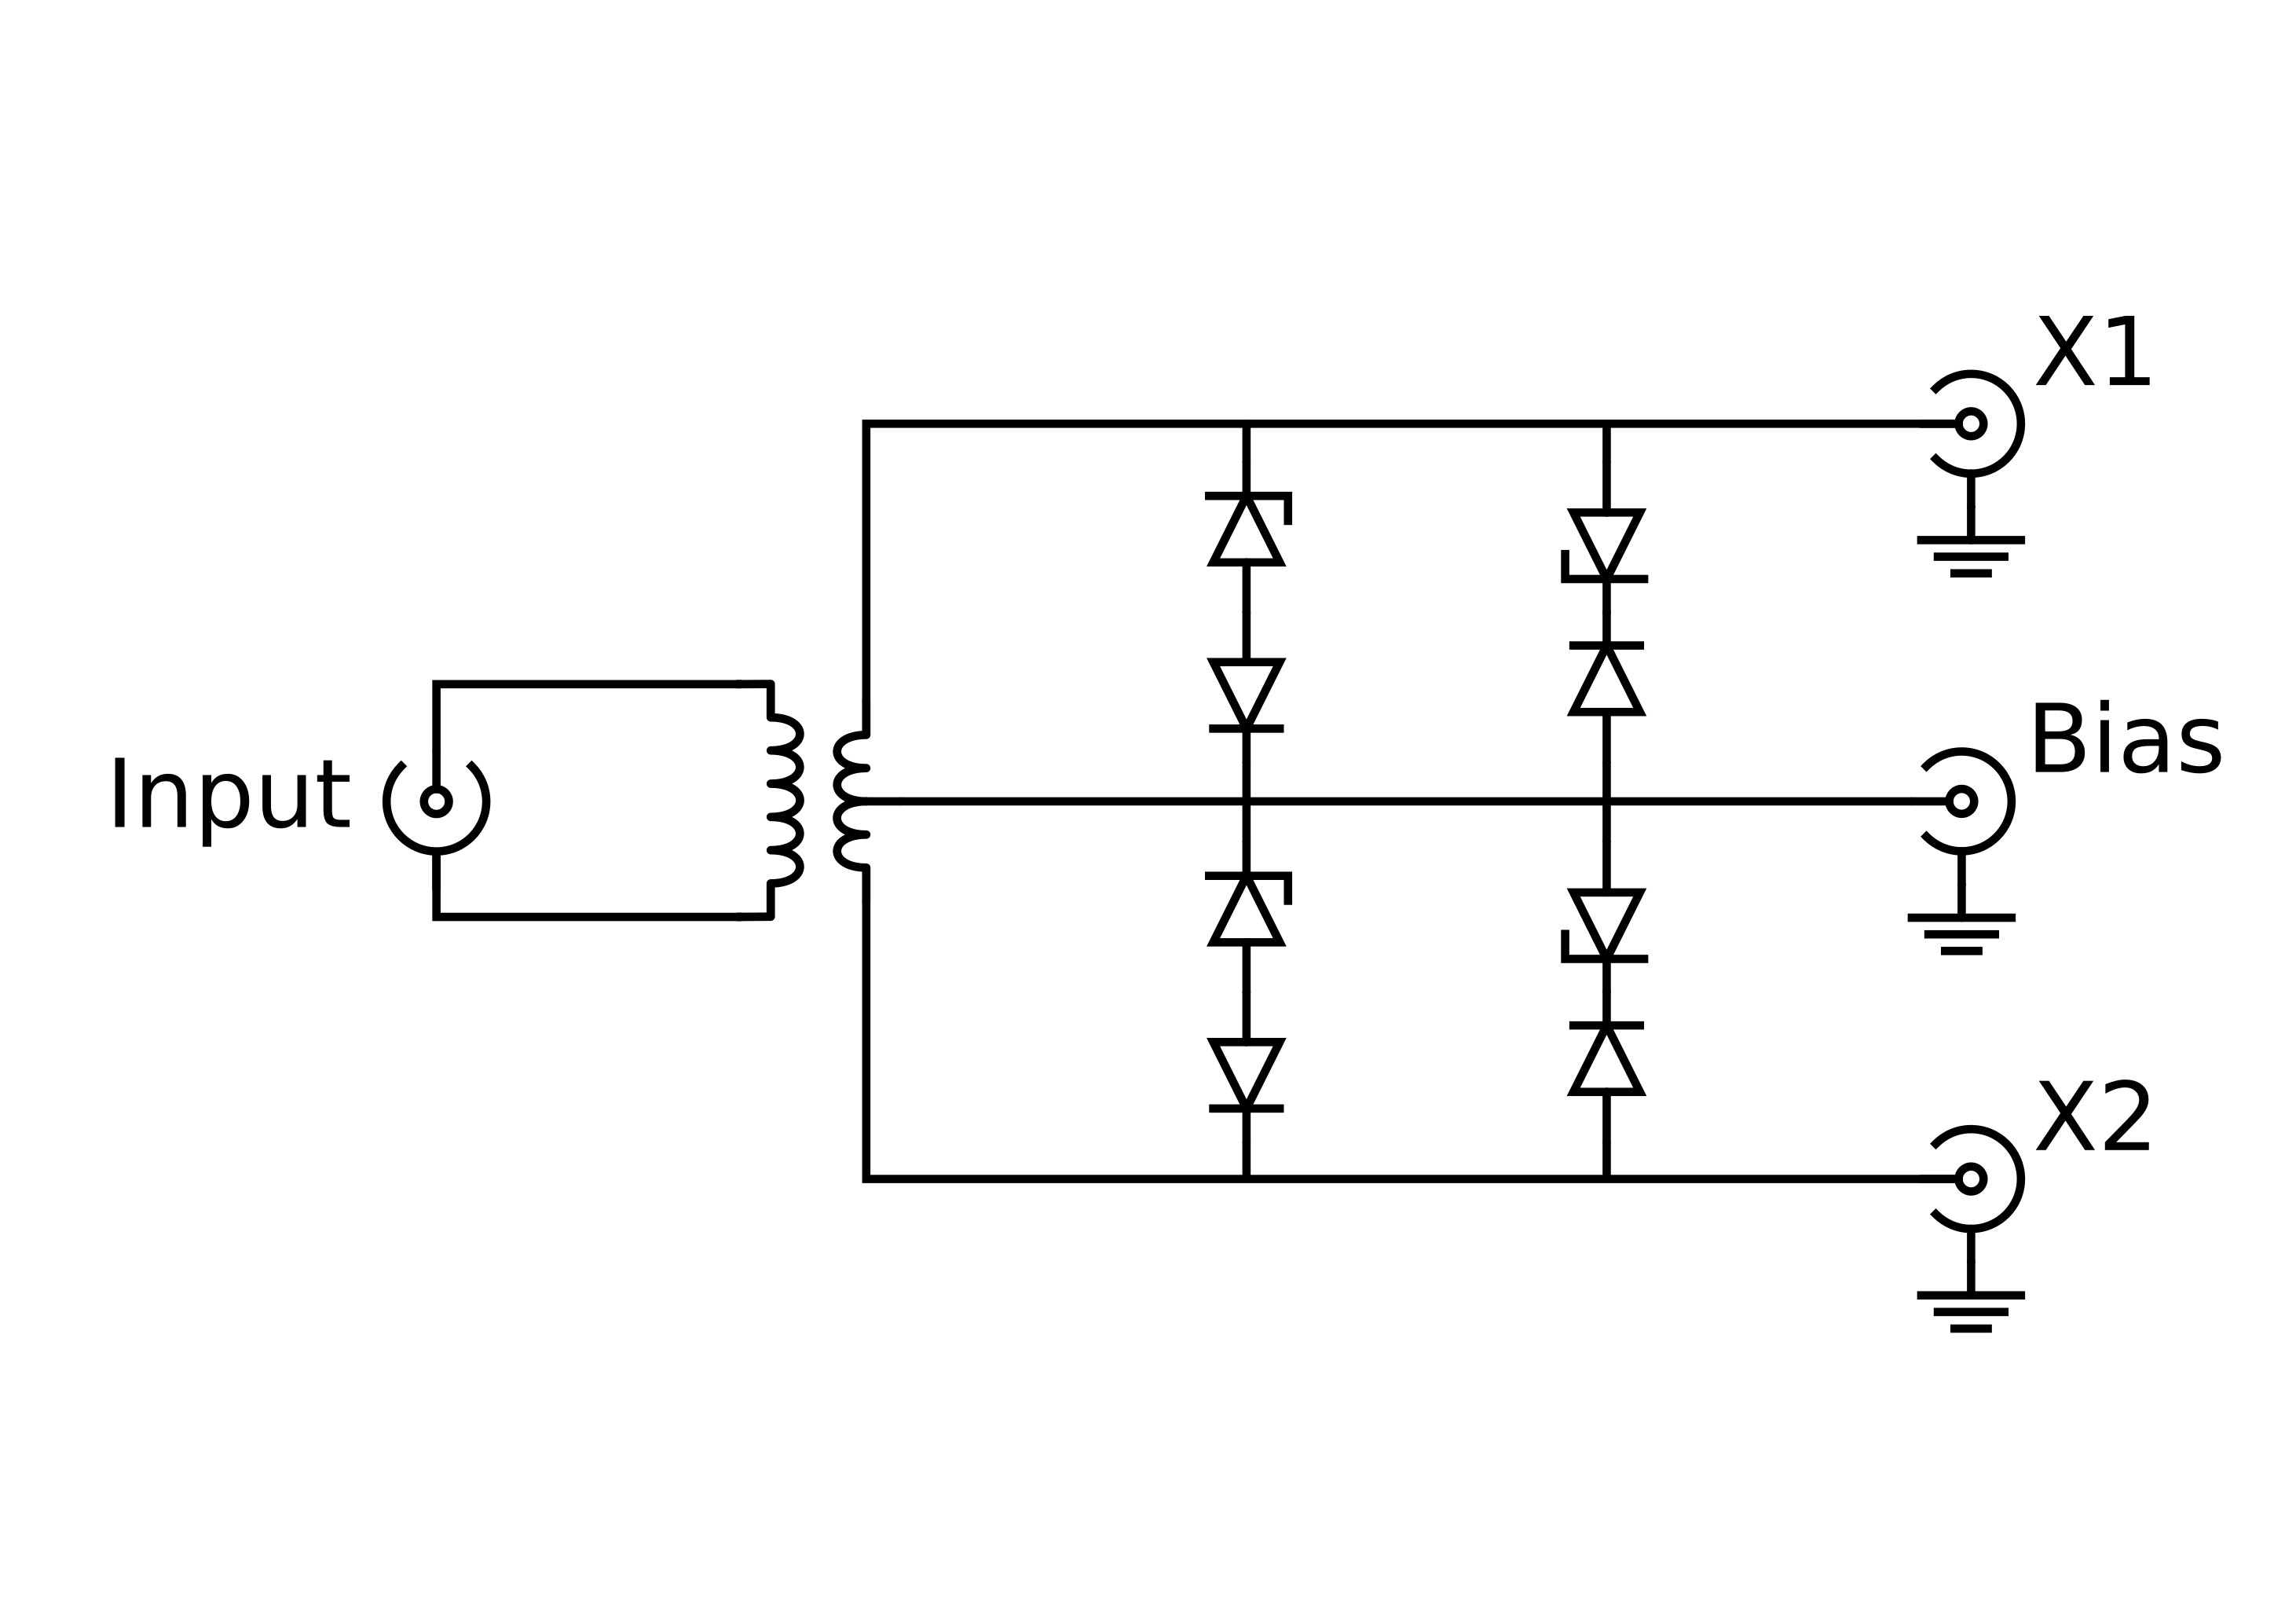
\includegraphics[height=0.2\textheight]{Chapters/Deflection/circuit_CTT}
	\caption{}
	\label{fig:circuit_ctt}
\end{subfigure}%
\begin{subfigure}{.5\textwidth}
	\centering
	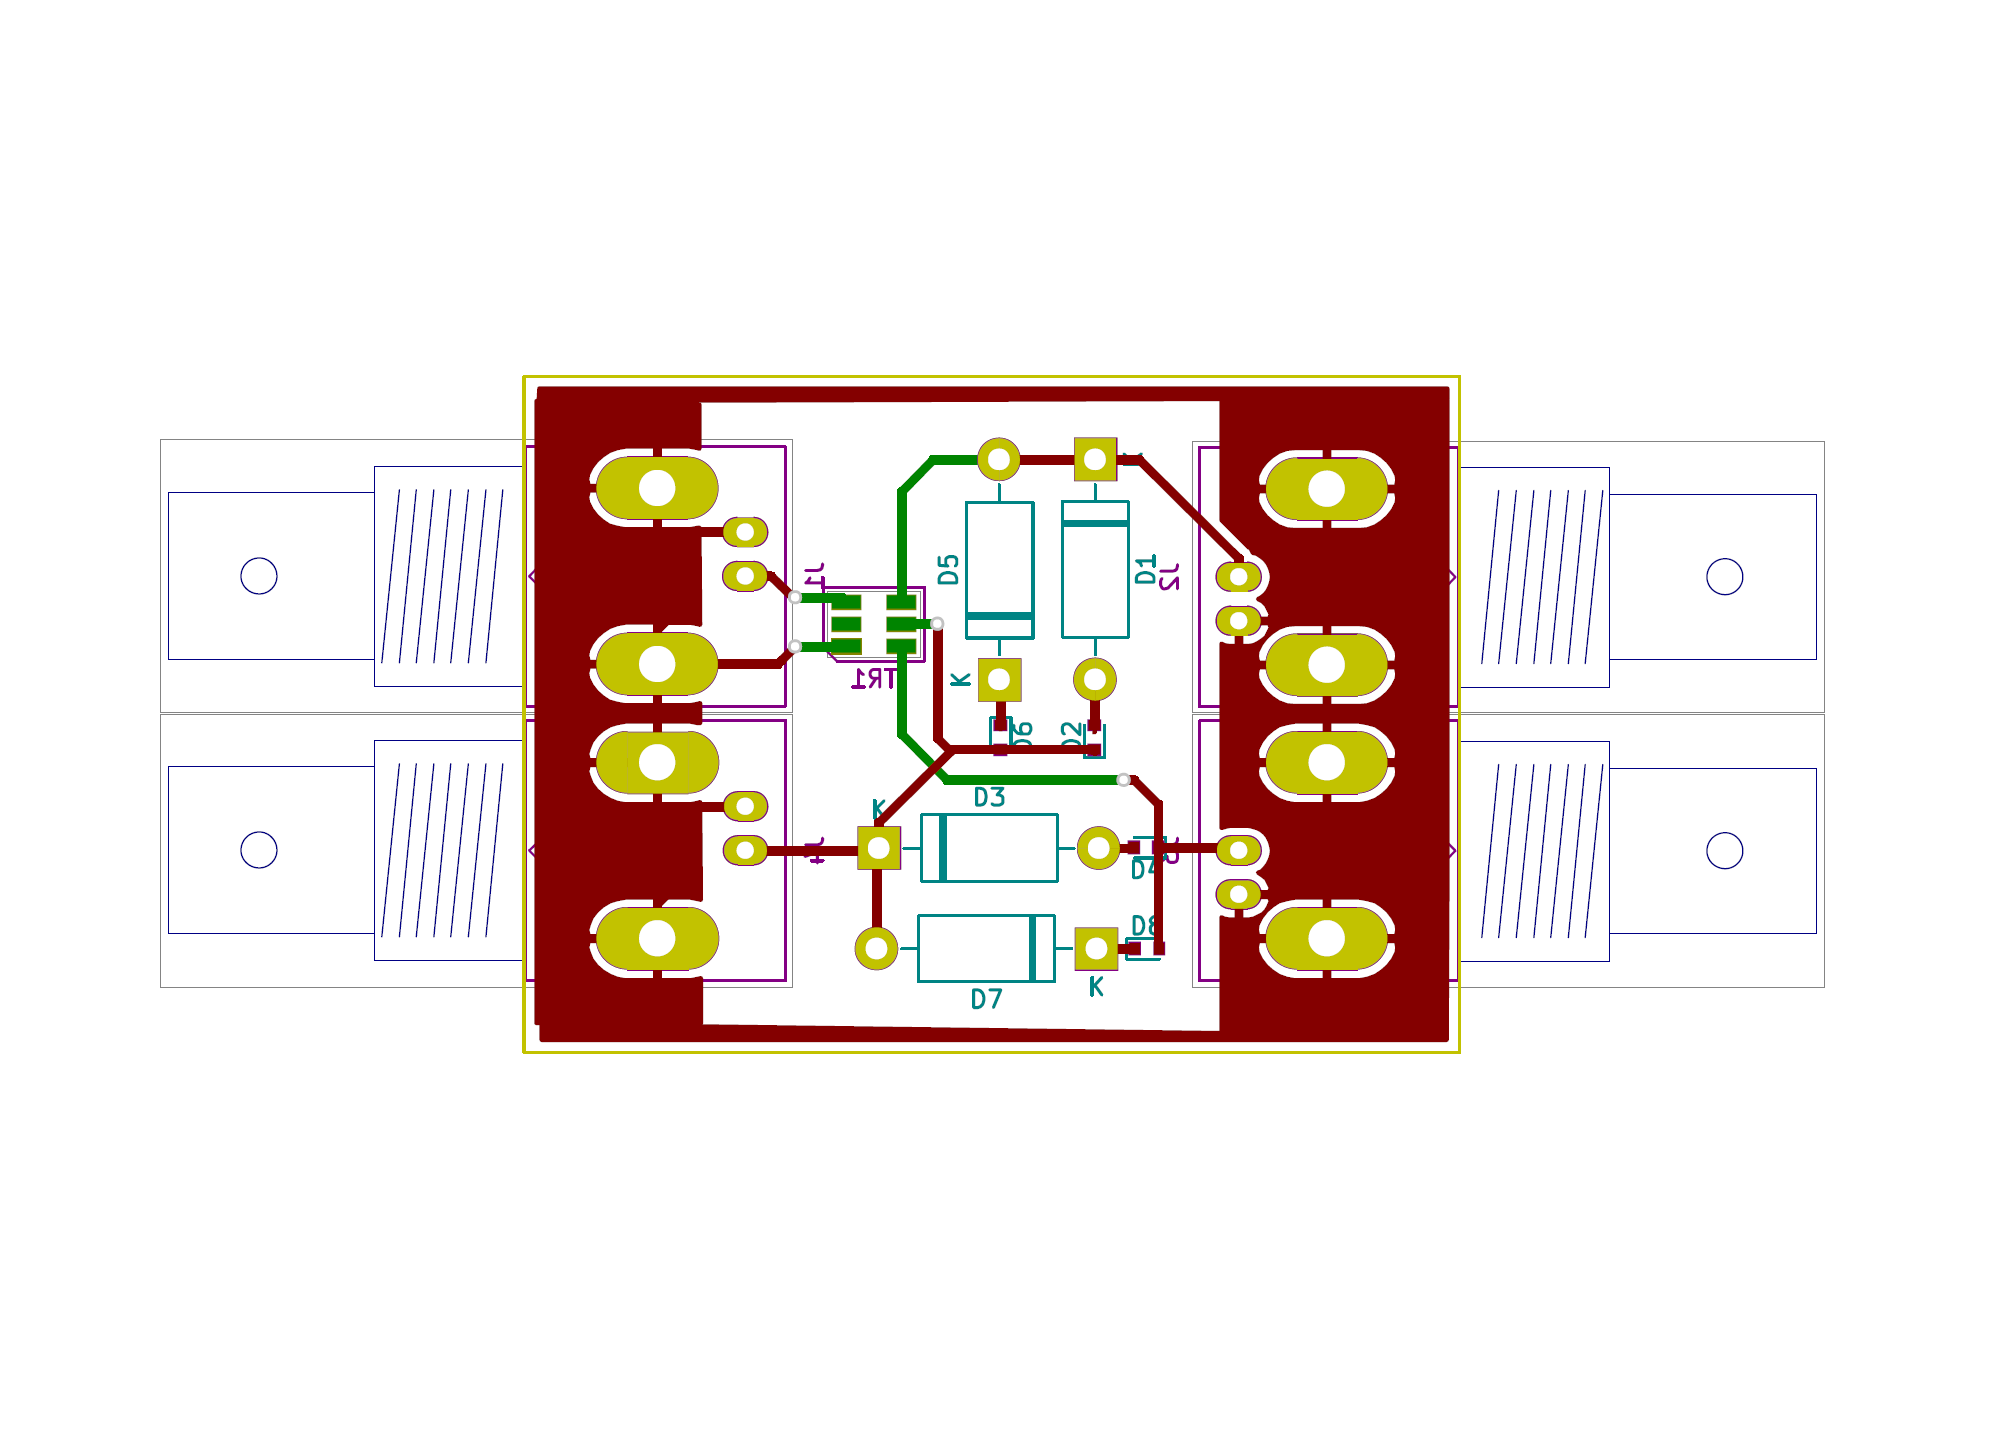
\includegraphics[height=0.2\textheight]{Chapters/Deflection/PCB_CTT}
	\caption{}
	\label{fig:PCB_CTT}
\end{subfigure}
\caption{}
\label{fig:CTT}
\end{figure}



